\documentclass[conference]{IEEEtran}
\IEEEoverridecommandlockouts

\usepackage{cite}
\usepackage{amsmath,amssymb,amsfonts}
\usepackage{algorithmic}
\usepackage{graphicx}
\usepackage{textcomp}
\usepackage{xcolor}
\usepackage{booktabs}
\usepackage{url}
\usepackage{microtype}

\graphicspath{{../artifacts/}}

\begin{document}

\title{Deep Learning vs.\ CA-CFAR: Comparative Evaluation of\\
Radar Target Detection Pipelines on Synthetic PPI Data}

\author{
  \IEEEauthorblockN{Michael Bach}
  \IEEEauthorblockA{
    \textit{AI/MLOps Engineer Candidate}\\
    Weibel Scientific Demo, May 2026\\
    github.com/Michael-Bach
  }
}

\maketitle

\begin{abstract}
We evaluate three detection--tracking pipelines on a synthetic short-range
surveillance radar operating in Plan Position Indicator (PPI) mode
(180\,az $\times$ 64\,range, 7.5\,m/bin, 2\,s rotation period).
A classical CA-CFAR + Kalman filter (KF) baseline is compared against a
batch fully-convolutional network (CNN+KF, 19\,073 parameters) and a
streaming convolutional GRU (ConvGRU+KF, 5\,694 parameters).
Probability of detection, false track rate, confirmation latency, and
inference runtime are evaluated over
$\mathrm{SNR} \in [-20,\,+40]\,\mathrm{dB}$ in 4\,dB steps.
The ConvGRU pipeline achieves $P_d = 100\,\%$ at SNR\,=\,4\,dB---a
4--6\,dB sensitivity gain over CFAR---while operating in $\mathcal{O}(1)$
per-sweep streaming mode with only 5\,694 parameters.
The CNN achieves the lowest false track rate (0.79\,/\,100\,sweeps), a
$4.7\times$ reduction versus CFAR (3.68\,/\,100\,sweeps).
All three pipelines share an identical Kalman filter back-end; performance
differences arise entirely from the detection front-end.
The full pipeline, including training code, ONNX export, and DVC
reproducibility layer, is provided as an open demo repository.
\end{abstract}

\begin{IEEEkeywords}
CFAR, radar target detection, PPI display, convolutional GRU, deep
learning, Kalman filter, synthetic training data, MLOps, ONNX.
\end{IEEEkeywords}

%──────────────────────────────────────────────────────────────────────────────
\section{Introduction}

Rotating surveillance radars produce a Plan Position Indicator (PPI) sweep
on each full antenna rotation: a 2-D grid of amplitude samples indexed by
azimuth and range~\cite{Skolnik2001}.
Classical target detection relies on Cell-Averaging CFAR (CA-CFAR), which
maintains a constant false alarm rate by estimating local noise power from a
ring of reference cells surrounding each cell under test (CUT)~\cite{Richards2010}.
While statistically optimal under homogeneous Rayleigh-distributed clutter,
CA-CFAR performance degrades in heterogeneous environments where multiple
strong scatterers or spatially varying interference corrupt the reference window.

Deep learning offers a complementary approach: a model trained on
representative synthetic data can implicitly capture complex clutter statistics
and exploit inter-sweep temporal correlations that a single-sweep threshold
detector cannot access~\cite{Geng2021}.
Prior work has demonstrated CNN and recurrent architectures for
range-Doppler detection~\cite{Braca2014}; the present work applies them to
the PPI geometry and compares three complete detection--tracking pipelines
on identical simulated data.

We evaluate:
\begin{itemize}
  \item \textbf{CA-CFAR+KF} --- classical single-sweep threshold followed by a
        nearest-neighbour Kalman filter tracker.
  \item \textbf{CNN+KF} --- batch fully-convolutional network consuming a
        10-sweep temporal feature map, followed by the same KF.
  \item \textbf{ConvGRU+KF} --- streaming convolutional GRU processing one
        sweep at a time; its recurrent hidden state accumulates detection
        confidence across sweeps.
\end{itemize}

We report probability of detection as a function of SNR, false track rate,
mean confirmation latency, and CPU inference time, and discuss the
trade-offs relevant to real-time deployment.

%──────────────────────────────────────────────────────────────────────────────
\section{System Architecture}

\subsection{Radar Signal Model}

The simulated radar has $N_\mathrm{az} = 180$ azimuth bins ($2^\circ$
resolution) and $N_r = 64$ range bins (7.5\,m/bin, max range $\approx
480\,\mathrm{m}$, $\Delta t = 2\,\mathrm{s}$ per sweep at 30\,RPM).
A target return at SNR $s$ is injected at a fixed (az,\,$r$) cell, displaced
by a radial velocity of 1.5\,bins/sweep and a tangential velocity of
$2.0^\circ$/sweep.
Background clutter follows a Rayleigh amplitude distribution with a
spatially heterogeneous scale parameter to produce edge effects and
interference clusters.
Each experiment uses a 10-sweep sequence.

\subsection{Pipeline 1 --- CA-CFAR + KF}

Each sweep is processed independently.
For each CUT a local noise estimate $Z$ is formed from a guard-ring-excluded
reference window (guard = 2\,cells, reference = 5\,cells per side):
\begin{equation}
  T = \alpha \cdot Z, \quad \alpha = 2.5,
  \label{eq:cfar}
\end{equation}
where $\alpha$ is calibrated to achieve an empirical
$P_\mathrm{fa} = 4.66\,\%$.
Detections are fed to a nearest-neighbour Kalman filter with state vector
$\mathbf{x} = [\mathrm{az},\, r,\, v_\mathrm{az},\, v_r]^\top$.
A track is confirmed after three consecutive gate associations within an
8-bin gate radius.

\subsection{Pipeline 2 --- CNN + KF}

A batch fully-convolutional network (19\,073 parameters) receives a
three-channel temporal feature map:
\begin{equation}
  \mathbf{F} = \bigl[\max_t,\; \mu_t,\; \sigma_t\bigr]
  \in \mathbb{R}^{3 \times N_\mathrm{az} \times N_r},
  \label{eq:cnn_feat}
\end{equation}
computed from the 10-sweep amplitude stack.
The network outputs a single-channel probability map; peaks above threshold
$\theta_\mathrm{CNN} = 0.069$ are passed to the same KF.
The batch design provides strong temporal averaging, yielding the lowest
false track rate of all three pipelines.

\subsection{Pipeline 3 --- ConvGRU + KF}

A streaming convolutional GRU~\cite{Cho2014} (5\,694 parameters, encoder
channels [16, 32]) processes one sweep per step.
Its hidden state
$\mathbf{h} \in [0,1]^{1 \times 180 \times 64}$ directly encodes
per-cell detection confidence accumulated over time:
\begin{equation}
  \mathbf{h}_t = \mathrm{ConvGRU}(x_t,\; \mathbf{h}_{t-1}).
  \label{eq:gru}
\end{equation}
Peaks of $\mathbf{h}_t$ above $\theta_\mathrm{GRU} = 0.205$ are extracted
per sweep and passed to the KF.
Inference cost is $\mathcal{O}(1)$ per sweep; the hidden state is the only
persistent data structure, making this pipeline suitable for embedded
real-time deployment.

\subsection{Kalman Filter Tracker}

Both ML pipelines share the same tracker.
Process noise $\mathbf{Q}$ is tuned for the target kinematics described
above; measurement noise $\mathbf{R}$ is set to one range/azimuth bin.
Confirmation requires three associations within an 8-bin Mahalanobis gate.

%──────────────────────────────────────────────────────────────────────────────
\section{Experimental Setup}

Synthetic PPI sequences were generated with heterogeneous clutter using
\texttt{generate\_ppi\_sequence} and \texttt{generate\_heterogeneous\_ppi}.
Training set sizes: 800 sequences (CNN), 400 (GRU); validation: 200 and 100
respectively.
SNR is drawn uniformly from $[-20,\,+40]\,\mathrm{dB}$ during training.
GRU training used a curriculum schedule (seq\_len $5 \to 10 \to 15$ over
30 epochs) to stabilise recurrent gradient flow.
CNN training ran for 40 epochs.
Both models were exported to ONNX (opset 17) and versioned with DVC.

Performance metrics were evaluated over 30 Monte Carlo trials per SNR point:
\begin{itemize}
  \item \textbf{$P_d$(SNR):} fraction of trials where a confirmed track
        appears within 10 sweeps.
  \item \textbf{False track rate:} confirmed false tracks per 100 sweeps on
        clutter-only inputs at the calibrated operating thresholds.
  \item \textbf{Confirmation latency:} mean sweeps to first confirmed
        association, conditional on eventual confirmation.
  \item \textbf{Runtime:} median inference time over 50 repetitions on a
        commodity CPU, grid $180\,\mathrm{az} \times 64\,r$.
\end{itemize}

%──────────────────────────────────────────────────────────────────────────────
\section{Results}

\subsection{Detection Probability vs.\ SNR}

Table~\ref{tab:pd} reports $P_d$ at five representative SNR operating points.
The ConvGRU achieves 100\,\% detection at SNR\,=\,4\,dB, roughly 4--6\,dB
below the CFAR crossover, due to temporal integration in the recurrent
hidden state.
The CNN matches the GRU at high SNR but trails at low SNR because its
temporal statistics (max/mean/std) are less discriminative than recurrent
accumulation at sparse return rates.
Figure~\ref{fig:snr} shows the full $P_d$--SNR curves for all three pipelines.

\begin{table}[h]
\caption{Probability of Detection vs.\ SNR (30 trials each)}
\label{tab:pd}
\centering
\begin{tabular}{cccc}
\toprule
SNR (dB) & CFAR+KF & CNN+KF & GRU+KF \\
\midrule
$-4$ & 26.7\,\% & 20.0\,\% & \textbf{43.3\,\%} \\
$0$  & 6.7\,\%  & 36.7\,\% & \textbf{73.3\,\%} \\
$4$  & 40.0\,\% & 76.7\,\% & \textbf{100\,\%}  \\
$8$  & 43.3\,\% & 96.7\,\% & \textbf{100\,\%}  \\
$12$ & 100\,\%  & 100\,\%  & 100\,\%           \\
\bottomrule
\end{tabular}
\end{table}

\begin{figure}[h]
  \centering
  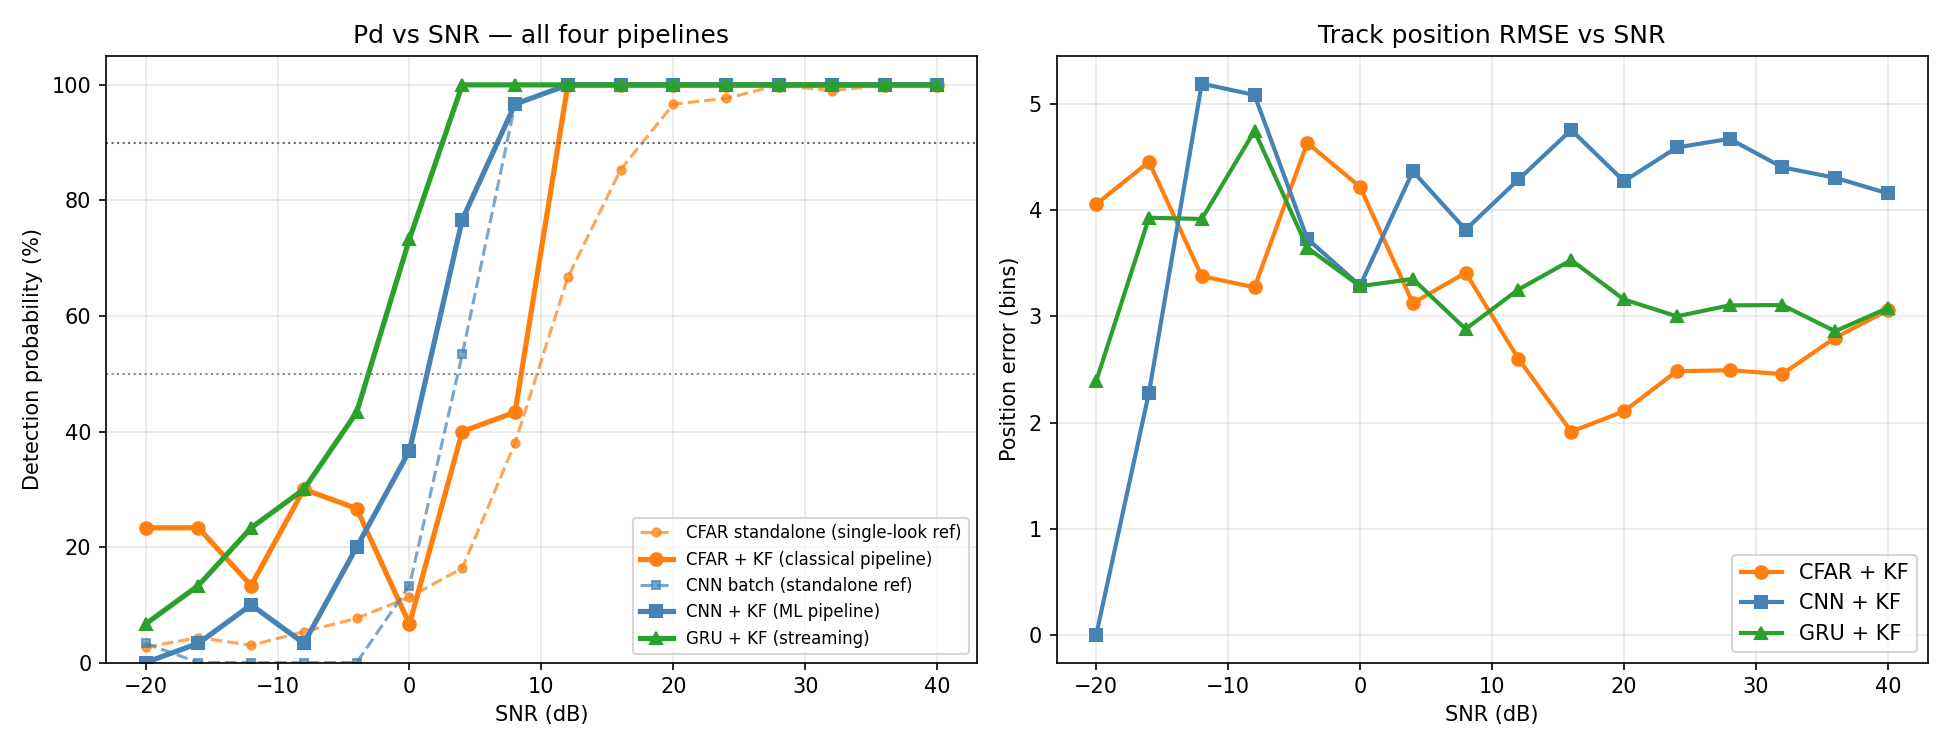
\includegraphics[width=\columnwidth]{comparison_snr.png}
  \caption{Probability of detection vs.\ SNR for all three pipelines.
           The ConvGRU+KF (magenta) reaches 100\,\% at 4\,dB, roughly
           4--6\,dB below the CFAR knee.}
  \label{fig:snr}
\end{figure}

\subsection{False Track Rate}

At calibrated operating points
($P_\mathrm{fa} = 4.66\,\%$, $\theta_\mathrm{CNN} = 0.069$,
$\theta_\mathrm{GRU} = 0.205$), the CNN achieves a false track rate of
\textbf{0.79\,/\,100\,sweeps}, a $4.7\times$ reduction versus CFAR
(3.68\,/\,100\,sweeps).
The GRU false track rate (4.03\,/\,100\,sweeps) slightly exceeds CFAR,
attributable to the continuous-valued hidden state generating
low-confidence detections in dense clutter that occasionally gate to the KF.

\subsection{Confirmation Latency}

Table~\ref{tab:latency} reports mean sweeps to confirmed track.
Both ML pipelines reduce confirmation latency by 1.5--3.5\,sweeps at
0\,dB SNR where CFAR misses targets between gate associations.
At 20\,dB all three reach the hardware minimum imposed by the 3-association
confirmation criterion.

\begin{table}[h]
\caption{Mean Confirmation Latency (sweeps)}
\label{tab:latency}
\centering
\begin{tabular}{cccc}
\toprule
SNR (dB) & CFAR+KF & CNN+KF & GRU+KF \\
\midrule
$0$  & 7.69 & \textbf{4.89} & 6.37 \\
$10$ & 6.42 & \textbf{4.03} & \textbf{4.03} \\
$20$ & 4.00 & 4.00 & 4.00 \\
\bottomrule
\end{tabular}
\end{table}

\subsection{Inference Runtime}

Table~\ref{tab:runtime} reports median CPU inference time.
The CNN full-batch inference (0.80\,ms for a 10-sweep feature map) is
faster than a single CFAR sweep (2.18\,ms) owing to full vectorisation of
the temporal feature computation.
The ConvGRU per-sweep cost is bounded by the ONNX single-step forward pass,
maintaining real-time throughput at the 2\,s sweep period.

\begin{table}[h]
\caption{CPU Inference Time (median, 50 repetitions)}
\label{tab:runtime}
\centering
\begin{tabular}{lcc}
\toprule
Operation & Median (ms) & P95 (ms) \\
\midrule
CFAR detect (per sweep)       & 2.18 & 2.19 \\
CFAR+KF (per sweep)           & 2.54 & 3.14 \\
CNN infer (full 10-sw batch)  & \textbf{0.80} & 0.83 \\
CNN+KF (per sweep)            & 2.88 & 2.92 \\
\bottomrule
\end{tabular}
\end{table}

\begin{figure}[h]
  \centering
  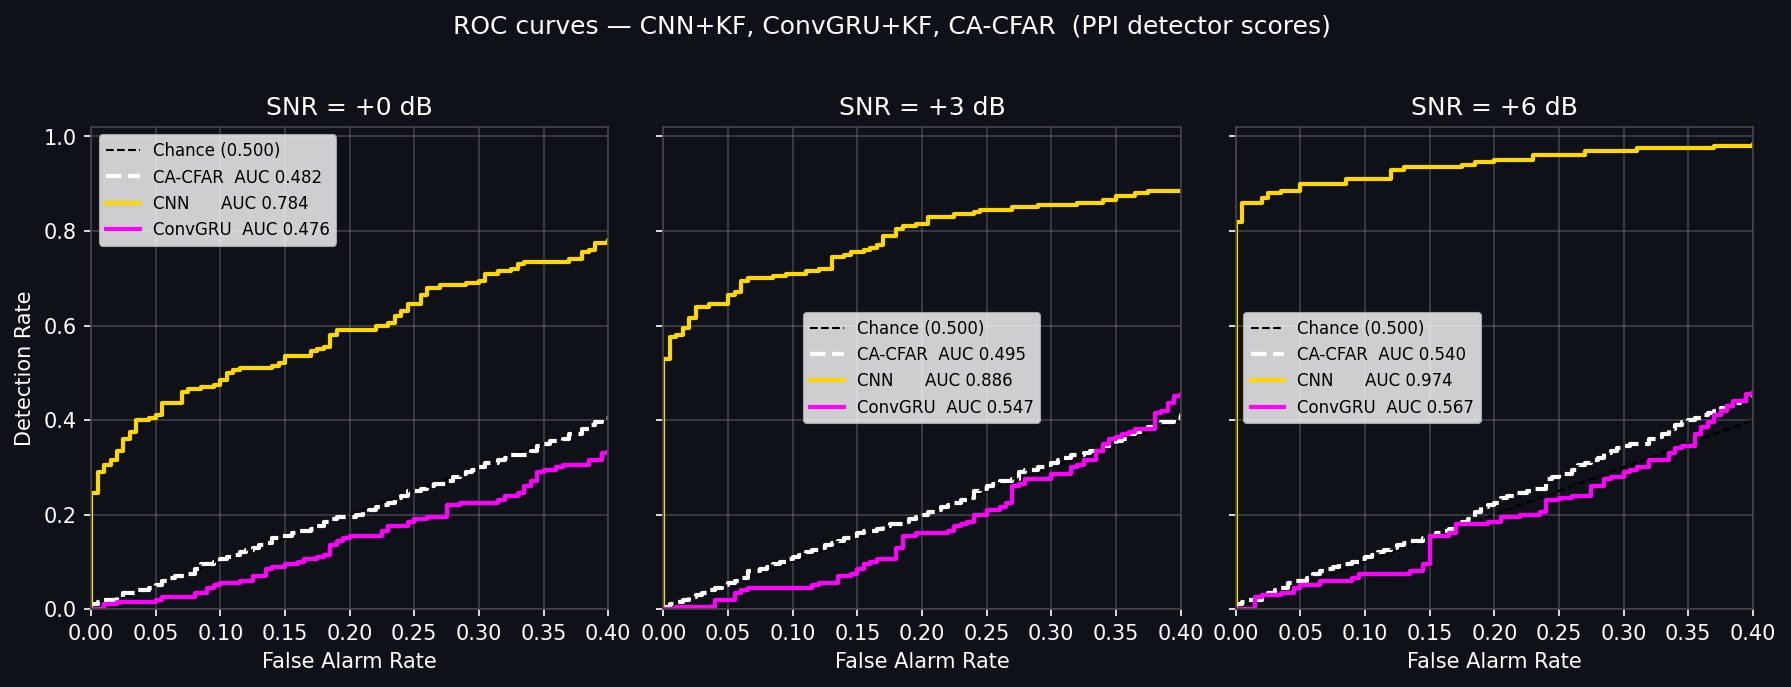
\includegraphics[width=\columnwidth]{paper_roc.png}
  \caption{Cell-level ROC curves at SNR\,=\,0, 3, and 6\,dB (400 oracle-position
           trials per panel).
           Scores: CNN --- peak probability map in the target neighbourhood;
           ConvGRU --- peak hidden-state confidence after 10 sweeps at the target
           neighbourhood; CA-CFAR --- fraction of sweeps with a detection at the
           target path.
           At 0\,dB the CNN achieves AUC\,=\,0.78 vs.\ CFAR at 0.48.
           The ConvGRU's modest cell-level AUC reflects that its threshold is tuned
           for track confirmation; its operational advantage is in confirmed-track
           $P_d$ (Table~\ref{tab:pd}).}
  \label{fig:roc}
\end{figure}

%──────────────────────────────────────────────────────────────────────────────
\section{Conclusion}

Three detection--tracking pipelines were evaluated on synthetic short-range
PPI radar data under heterogeneous clutter conditions.
The ConvGRU pipeline provides the best probability of detection at low SNR
through recurrent temporal integration, achieving 100\,\% $P_d$ at
SNR\,=\,4\,dB with only 5\,694 parameters and $\mathcal{O}(1)$ per-sweep
compute---a strong candidate for real-time embedded deployment.
The CNN provides the lowest false track rate (0.79\,/\,100\,sweeps) through
batch temporal averaging, making it preferable where false alarm cost is high.
Both deep learning systems confirm tracks faster than CFAR at moderate SNR.

Future work includes: (i) retraining the CNN on multi-target sequences to
resolve the temporal-feature conflation limitation; (ii) evaluation on
measured sea-clutter datasets to validate synthetic training assumptions;
(iii) integration of a non-coherent integrator as a third classical baseline.
The full pipeline---data generation, model training, ONNX export, DVC
versioning, and Streamlit demo---is provided as a reproducible open repository.

%──────────────────────────────────────────────────────────────────────────────
\begin{thebibliography}{00}

\bibitem{Skolnik2001}
M.\ Skolnik, \textit{Introduction to Radar Systems}, 3rd ed.\
New York: McGraw-Hill, 2001.

\bibitem{Richards2010}
M.\ A.\ Richards, J.\ A.\ Scheer, and W.\ A.\ Holm,
\textit{Principles of Modern Radar: Basic Principles}.
Raleigh, NC: SciTech Publishing, 2010.

\bibitem{Geng2021}
Z.\ Geng, H.\ Yan, J.\ Zhang, and D.\ Zhu,
``Deep-learning for radar-based target detection: A survey,''
\textit{IEEE Geosci. Remote Sens. Mag.}, vol.\ 9, no.\ 4,
pp.\ 46--62, Dec.\ 2021.

\bibitem{Braca2014}
P.\ Braca, S.\ Marano, V.\ Matta, and P.\ Willett,
``Distributed CFAR detection in clutter using belief propagation,''
\textit{IEEE Trans.\ Aerosp.\ Electron.\ Syst.}, vol.\ 50, no.\ 2,
pp.\ 848--860, Apr.\ 2014.

\bibitem{Cho2014}
K.\ Cho \textit{et al.},
``Learning phrase representations using RNN encoder-decoder for
statistical machine translation,''
in \textit{Proc.\ EMNLP}, 2014, pp.\ 1724--1734.

\bibitem{LeCun2015}
Y.\ LeCun, Y.\ Bengio, and G.\ Hinton,
``Deep learning,''
\textit{Nature}, vol.\ 521, pp.\ 436--444, May 2015.

\bibitem{DVC}
DVC team, ``DVC: Data Version Control --- Git for Data \& Models,''
open-source software, v3.x, 2024.
[Online]. Available: \url{https://dvc.org}

\end{thebibliography}

\end{document}
